\documentclass{eecslides}
\usepackage{amsmath}

%------------------------------
% PAGE TITRE

\title[Forêts-CC]{Des changements abruptes à prévoir pour les forêts du Pic Champlain?}
\subtitle{Vers une nouvelle génération de modèles de dynamique forestière}
\author[D. Gravel]{Dominique Gravel}
\institute[Chaire de recherche EEC]{UQAR -- Chaire de Recherche EEC}
\website{http://www.chaire-eec.uqar.ca/}
\date{\today}

\begin{document}

%------------------------------

	\begin{frame}[plain]
		\titlepage
	\end{frame}
	
%-------------------------------------------------------------------------------
%-------------------------------------------------------------------------------
	\section{Introduction}
%-------------------------------------------------------------------------------
%-------------------------------------------------------------------------------

	\begin{frame}
		\begin{center}
			\includegraphics[height=0.65\textheight]{Mckenney2007}
		\end{center}
	\end{frame}

%------------------------------

	\begin{frame}{Enveloppes climatiques}
		\begin{columns}
			\begin{column}{0.5\textwidth}
				\begin{center}
					\includegraphics[height=0.5\textheight]{Boulangeat2012}
				\end{center}
			\end{column}
%----
			\begin{column}{0.5\textwidth}
			De nombreuses suppositions
				\begin{itemize}
					\item Distribution à l'équilibre avec le climat;
					\item Aucune démographie;
					\item Aucune interaction biotique;
					\item Aucune limite à la dispersion;
					\item Réponse linéaire et instantanée au changement climatique;					
				\end{itemize}
			\end{column}
		\end{columns}	    	
	\end{frame}

%------------------------------

	\begin{frame}{Au Ministère des ressources naturelles}
		\begin{center}
			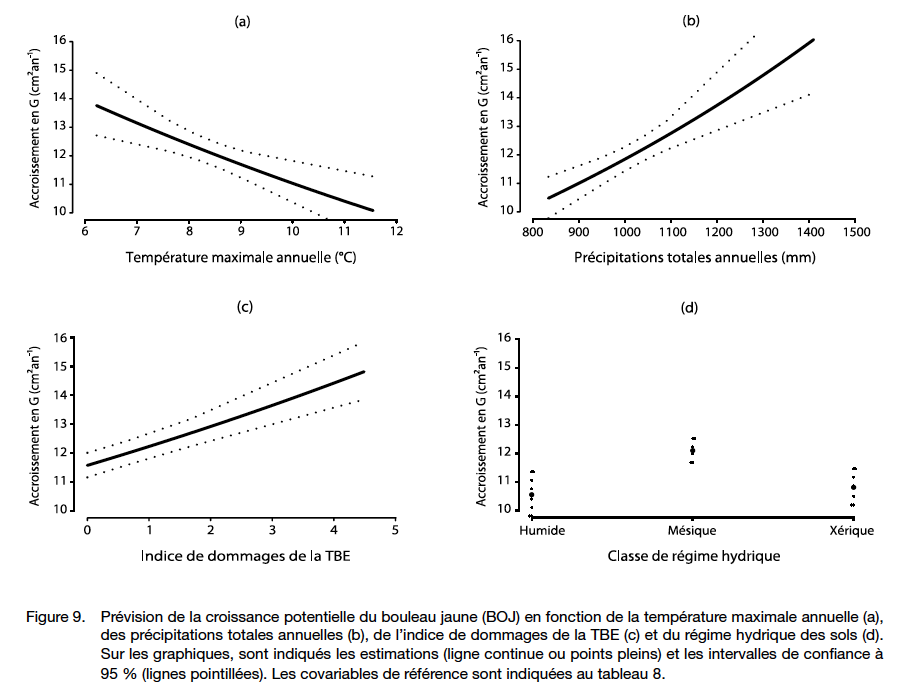
\includegraphics[height=0.65\textheight]{Perie2012.png}
		\end{center}
	\end{frame}

%------------------------------

	\begin{frame}

		\textit{Les outils actuels pour prédire l'impact des changements climatiques sur les écosystèmes forestiers sont limités par l'absence de processus écologiques fondamentaux.}

	\end{frame}
							
%-------------------------------------------------------------------------------
%-------------------------------------------------------------------------------
	\section{Objectifs}
%-------------------------------------------------------------------------------
%-------------------------------------------------------------------------------
	\begin{frame}{Objectifs}

		\textbf{Objectif général}: Prédire les impacts à court et long terme d'un changement climatique sur l'état et la productivité des forêts de l'Est du Canada. 
		\vskip 3em

		\textbf{Objectifs spécifiques}: 
		\begin{enumerate} 

			\item Développer de nouveaux outils de modélisation pour améliorer les prédictions de l'impact des changements climatiques sur les écosystèmes forestiers;
			\item Développer de nouvelles aproches pour estimer les risques et incertitudes;
			\item Évaluer l'aptitude de différentes stratégies d'aménagement forestier à minimiser les impacts négatifs des changements climatiques. 

		\end{enumerate}
	\end{frame}

%-------------------------------------------------------------------------------
%-------------------------------------------------------------------------------
	\section{Théorie}
%-------------------------------------------------------------------------------
%-------------------------------------------------------------------------------
	
	\begin{frame}{Contexte théorique}
		\begin{center}
		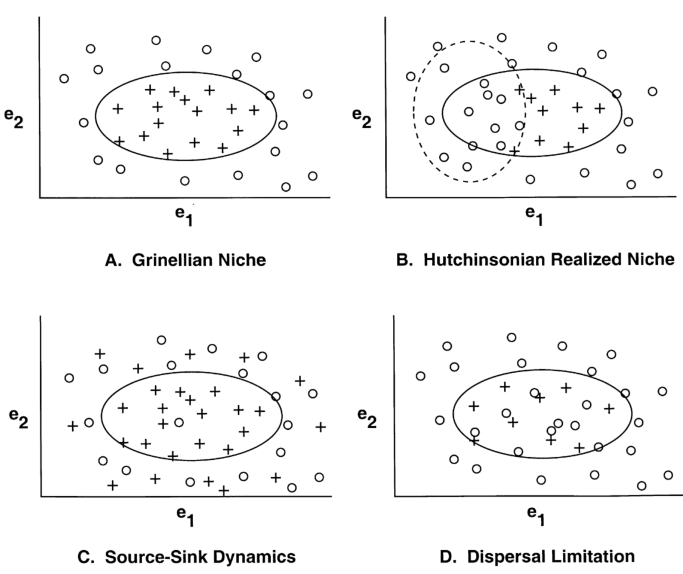
\includegraphics[height=0.6\textheight]{pulliam}\\
		\end{center}
	\end{frame}

%-------------------------------------------------------------------------------

	\begin{frame}{Contexte théorique}
		\begin{center}
		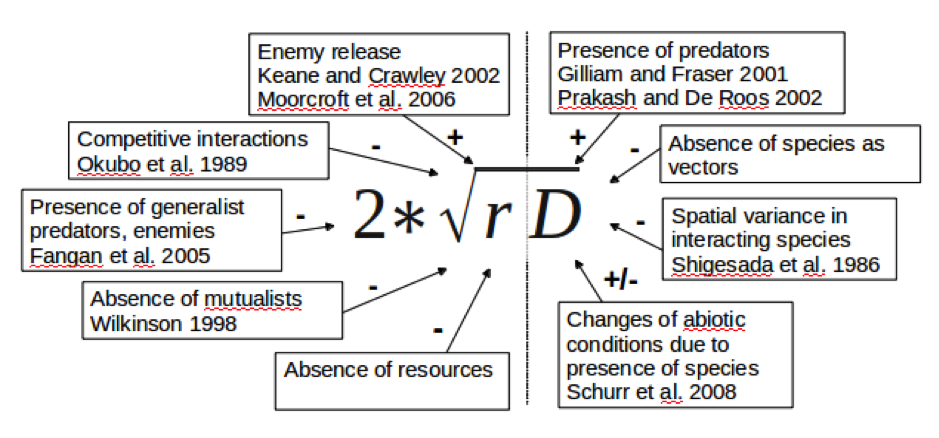
\includegraphics[height=0.6\textheight]{svenning}\\
		\end{center}
	\end{frame}

%-------------------------------------------------------------------------------

	\begin{frame}{Contexte théorique}
		\begin{center}
%		\includegraphics[height=0.6\textheight]{schaffer}\\
		\end{center}
	\end{frame}

%-------------------------------------------------------------------------------

	\begin{frame}{Contexte théorique}
		\begin{center}
		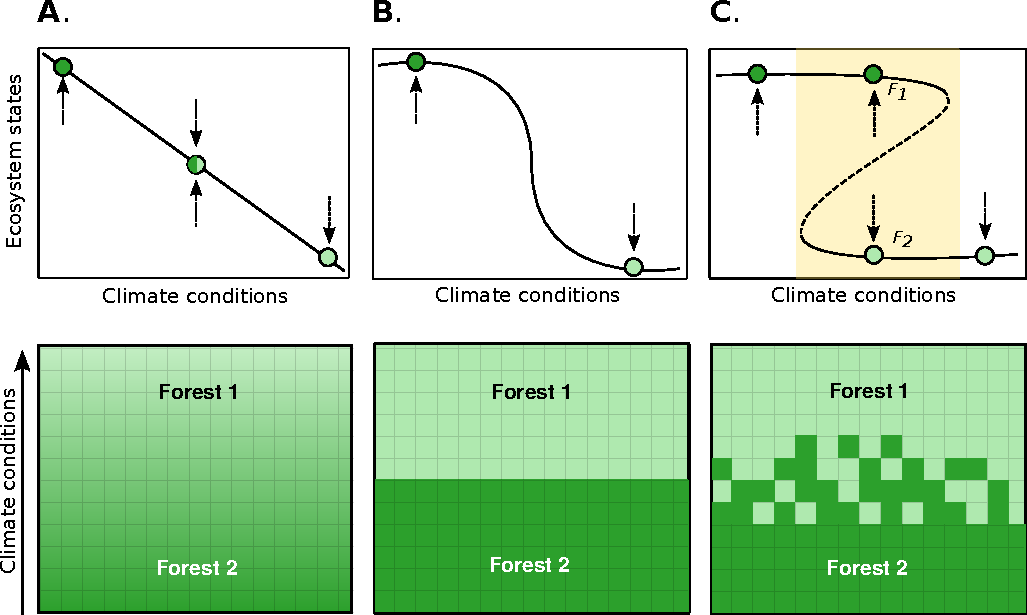
\includegraphics[height=0.6\textheight]{states}\\
		\end{center}
	\end{frame}

%-------------------------------------------------------------------------------

	\begin{frame}{Contexte théorique}
		\begin{center}
		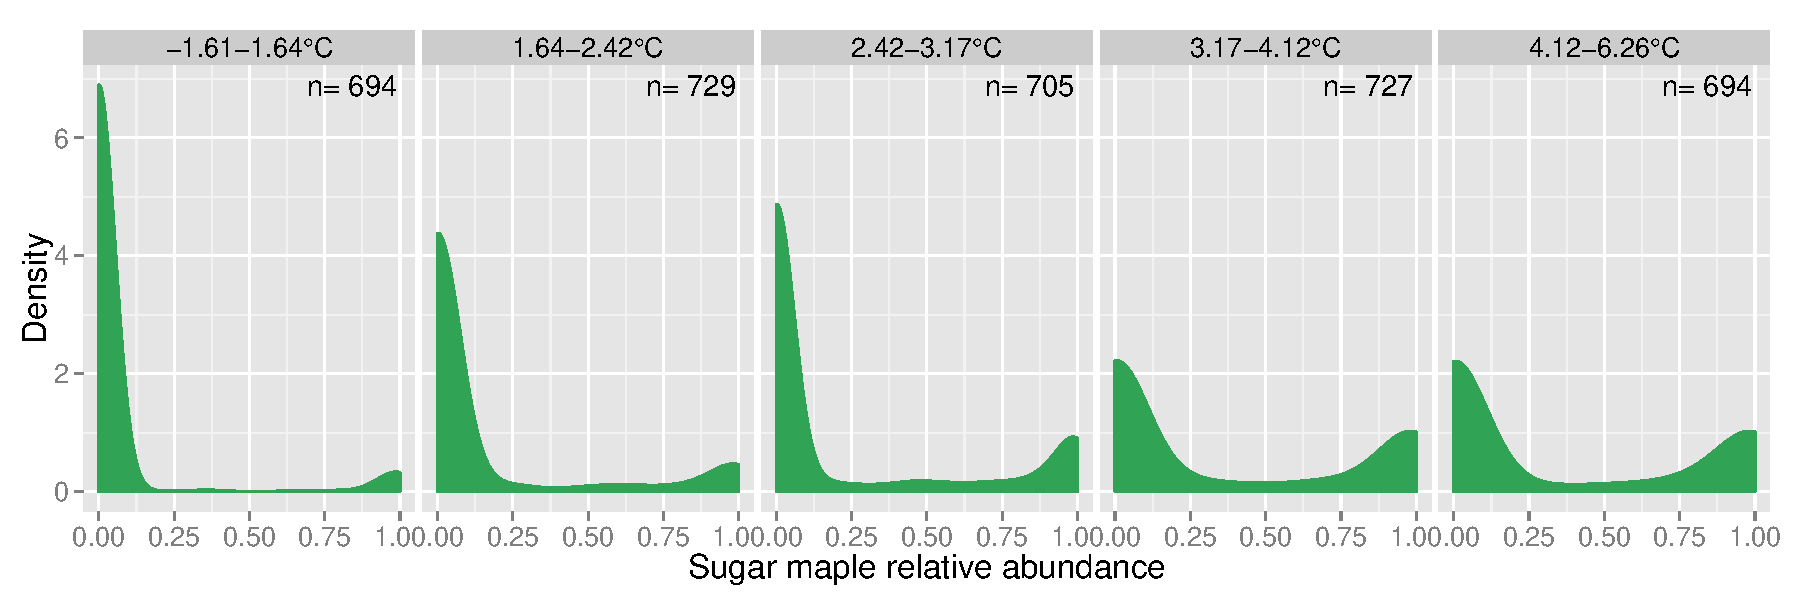
\includegraphics[height=0.6\textheight]{ass_ers}\\
		\end{center}
	\end{frame}

%-------------------------------------------------------------------------------
%-------------------------------------------------------------------------------
	\section{Projet}
%-------------------------------------------------------------------------------
%-------------------------------------------------------------------------------
	
	\begin{frame}{Description du projet}{Volet 1}
		\textbf{Objectif}: Développer notre compréhension théoriques des facteurs qui affectent la migration des arbres sous l'effet des changements climatiques

		\begin{center}
			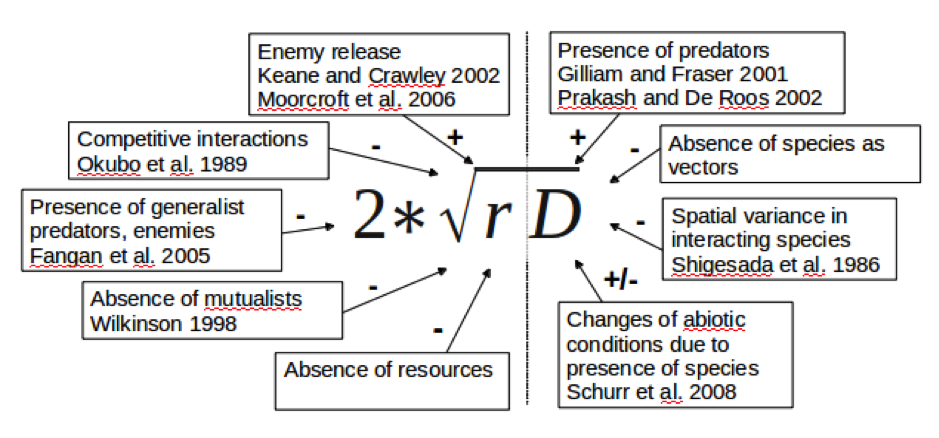
\includegraphics[height=0.5\textheight]{svenning.png}
		\end{center}

	\end{frame}

%-------------------------------------------------------------------------------
	
	\begin{frame}{Description du projet}{Volet 2}

	\textbf{Objectif}: Développer des modèles démographiques dépendant du climat

		\begin{enumerate}
			\item Croissance, mortalité et compétition;  
			\item Représenter spatialement les impacts à court terme sur la productivité;
			\item Tester si la diversité a un effet positif sur l'adaptation. 
		\end{enumerate}
		
	\end{frame}

%-------------------------------------------------------------------------------
	
	\begin{frame}{Description du projet}{Volet 3}
	\textbf{Objectif}: Développer une suite intégrée de modèles, de l'arbre jusqu'au continent 

		\begin{enumerate}
			\item Modèle de peuplement dépendant du climat;
			\item Modèle de paysage dépendant du climat;
			\item Cartographie de la distribution et productivité future;
			\item Comparaison des taux de migration entre modèles;
			\item Couplage avec les espèces herbacées et les herbivores.
		\end{enumerate}
	\end{frame}

%-------------------------------------------------------------------------------
	
	\begin{frame}{Description du projet}{Volet 4}

	\textbf{Objectif:} Évaluer de nouvelles stratégies d'aménagement forestier et de conservation

		\begin{enumerate}
			\item Business as usual;
			\item Migration assistée;
			\item Couloirs de migration;
			\item Sylviculture haute diversité;
			\item Anticipation des changements de composition.	
		\end{enumerate}
	\end{frame}

%-------------------------------------------------------------------------------
%-------------------------------------------------------------------------------
\section{Méthodes}
%-------------------------------------------------------------------------------
%-------------------------------------------------------------------------------

	\begin{frame}{Base de données}
		\begin{enumerate}
			\item Parcelles échantillons temporaires (MRNQ);
			\item Parcelles échantillons permanentes (MRNQ)
			\item Domtar;
			\item OMNR;
			\item Nouveau-Brunswick;
			\item FIA.
		\end{enumerate}
	\end{frame}

%-------------------------------------------------------------------------------

	\begin{frame}{Large parcelles permanentes}
		\begin{columns}
			\begin{column}{0.5\textwidth}
				\begin{center}
					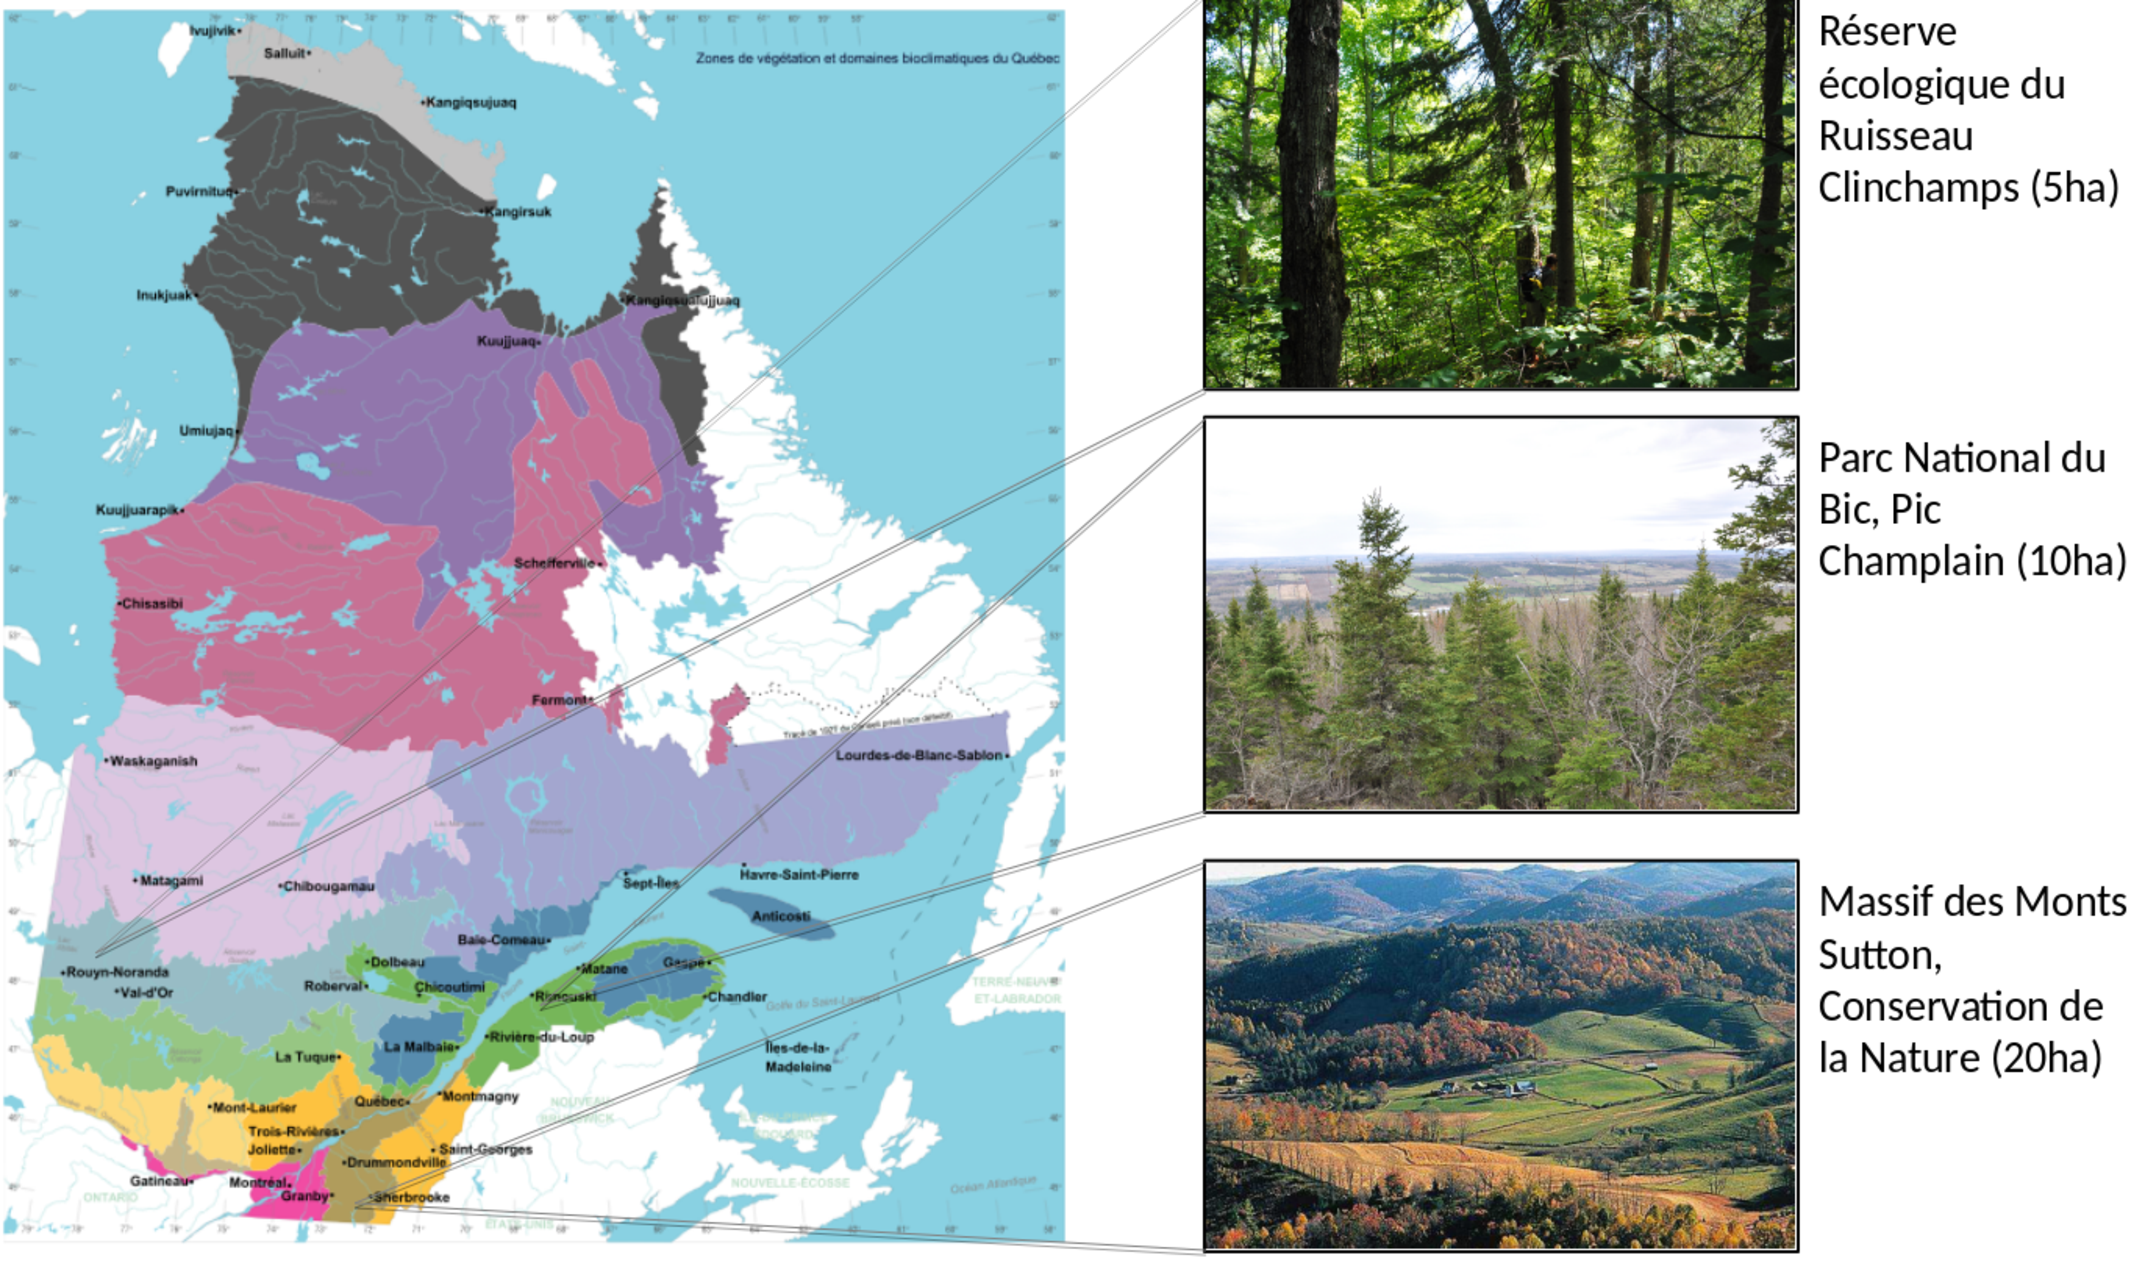
\includegraphics[height=0.5\textheight]{carte_parcelles}
				\end{center}
			\end{column}
%----
			\begin{column}{0.5\textwidth}
			Mesures:
				\begin{itemize}
					\item Coordonnées des arbres;
					\item Diamètre;
					\item Espèce;			
					\item Regénération;
					\item Senseurs de température;
					\item Mesures d'humidité;
					\item Pièges fosse;
					\item Germination (expérience en parallèle sur 15 sites).
				\end{itemize}
			\end{column}
		\end{columns}	    	
	\end{frame}

%-------------------------------------------------------------------------------

	\begin{frame}{Parcelle du Pic Champlain}
				\begin{center}
					\includegraphics[height=0.5\textheight]{carte_Bic}
				\end{center}
	\end{frame}

%-------------------------------------------------------------------------------

	\begin{frame}{Parcelle du Pic Champlain}
		\begin{columns}
			\begin{column}{0.5\textwidth}
				\begin{center}
					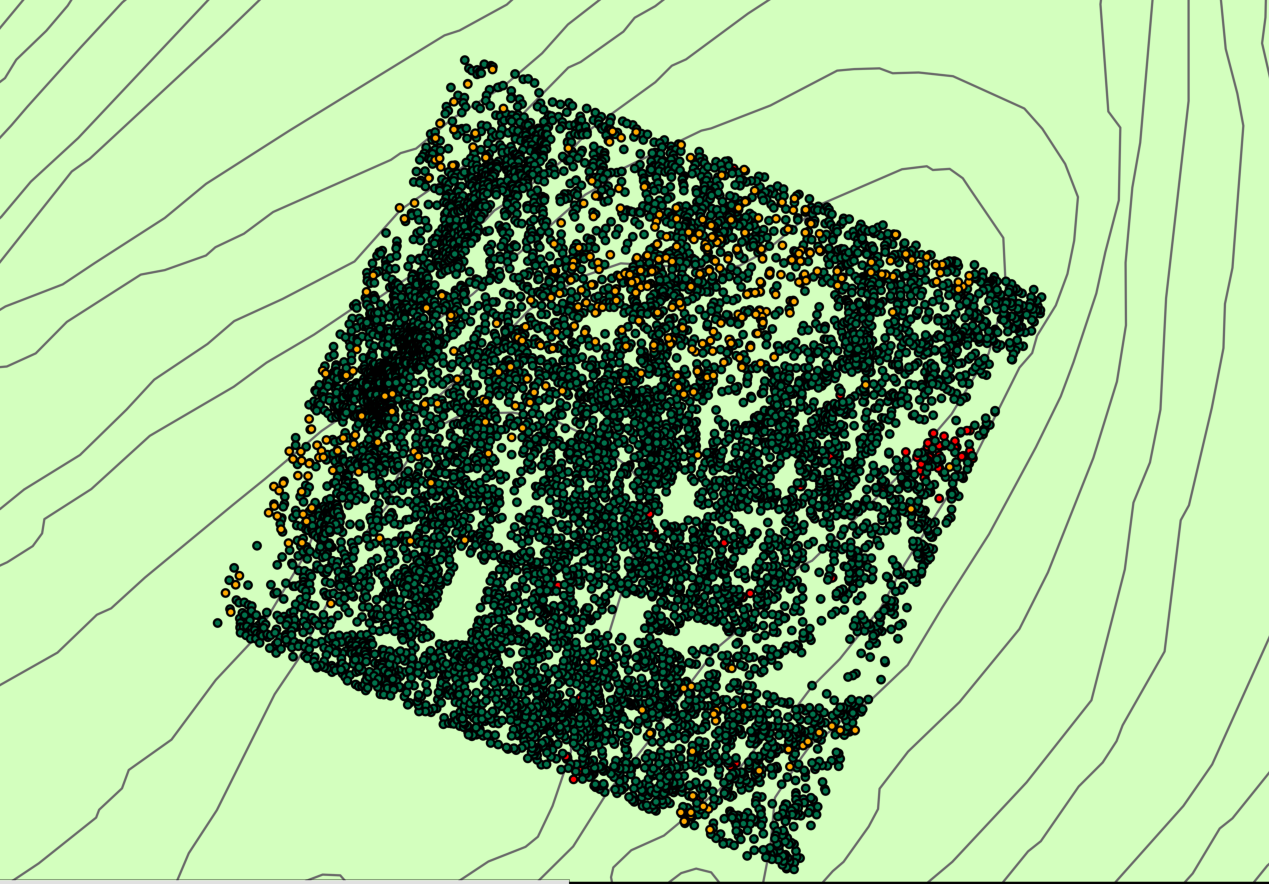
\includegraphics[height=0.5\textheight]{carte_arbres}
				\end{center}
			\end{column}
%----
			\begin{column}{0.5\textwidth}
				\begin{center}
					\includegraphics[height=0.5\textheight]{tableau_especes}
				\end{center}
			\end{column}
		\end{columns}	    	
	\end{frame}

%-------------------------------------------------------------------------------
%-------------------------------------------------------------------------------
\section{Résultats}
%-------------------------------------------------------------------------------
%-------------------------------------------------------------------------------

	\begin{frame}{Modèle}
		\begin{center}
			\includegraphics[height=0.5\textheight]{modele}
		\end{center}
	\end{frame}

%-------------------------------------------------------------------------------

		\begin{frame}{Distribution}
		\begin{columns}
			\begin{column}{0.5\textwidth}
				Distribution actuelle des états
								\begin{center}
					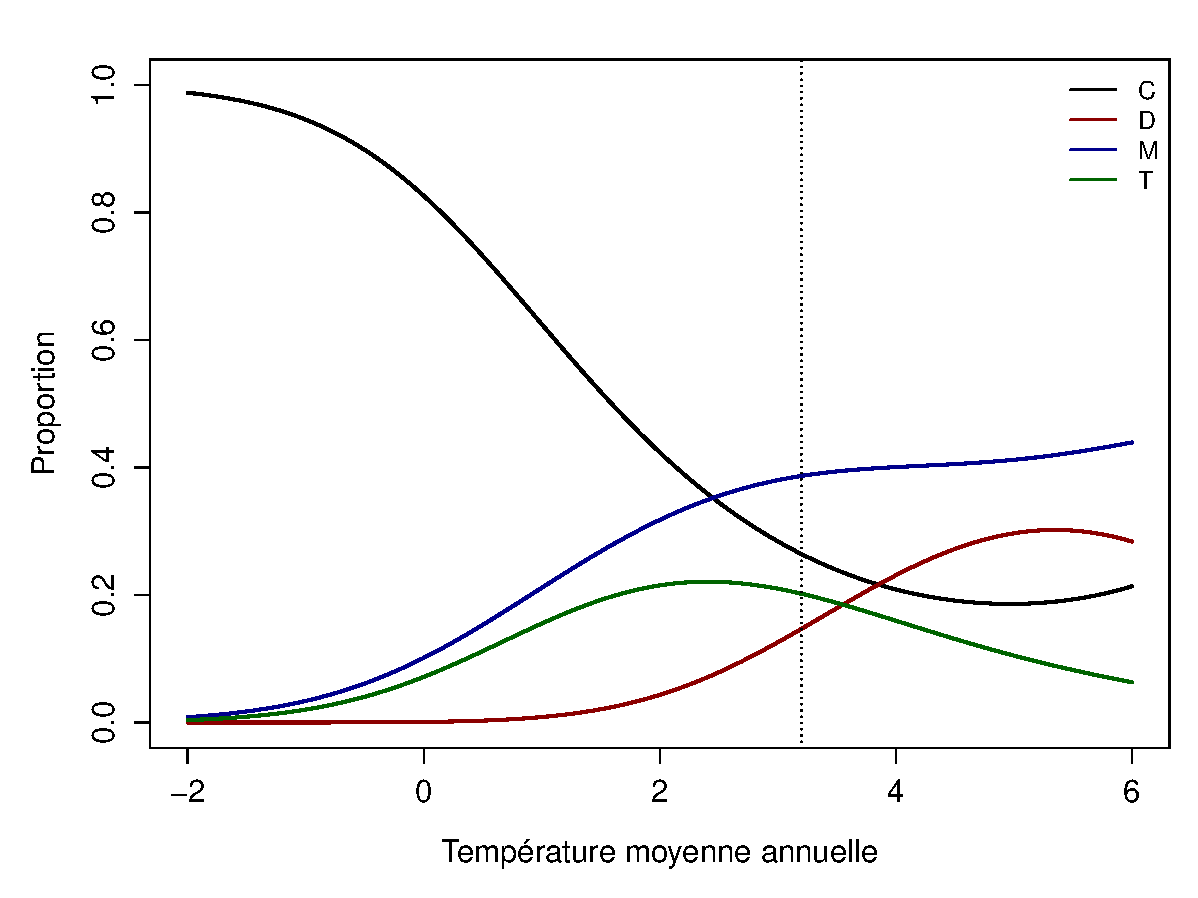
\includegraphics[height=0.5\textheight]{SDM}
				\end{center}
			\end{column}----
%----
			\begin{column}{0.5\textwidth}
				Distribution modélisée
				\begin{center}
					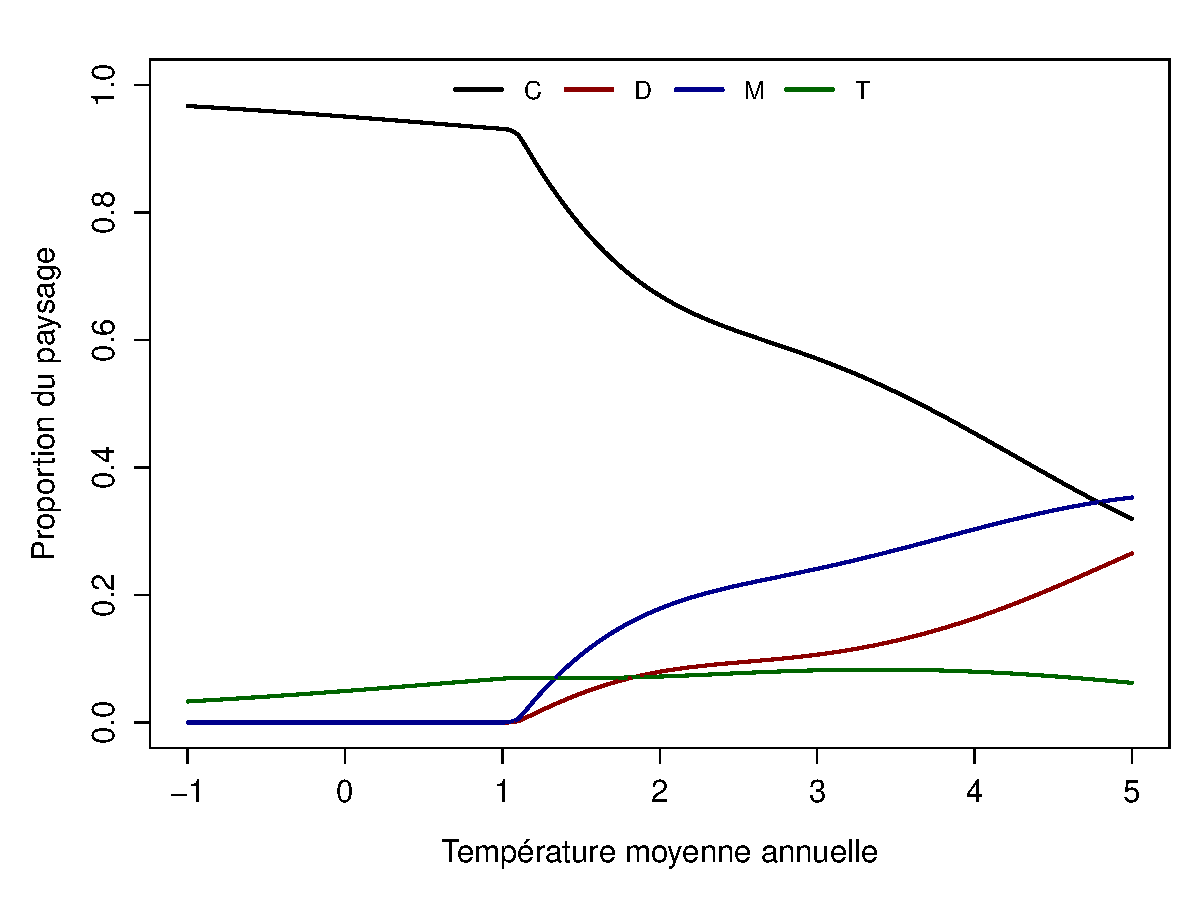
\includegraphics[height=0.5\textheight]{SDMeq}
				\end{center}
			\end{column}
		\end{columns}	    	
	\end{frame}

%-------------------------------------------------------------------------------

	\begin{frame}{Et si on monte la température...}
		% Proportion D au fil du temps
	\end{frame}

%-------------------------------------------------------------------------------

	\begin{frame}{Et sur le Pic Champlain}
	% Carte au T0

	\end{frame}

%-------------------------------------------------------------------------------

	\begin{frame}{Et sur le Pic Champlain}
	% Carte après 100 ans
	\end{frame}

%-------------------------------------------------------------------------------

	\begin{frame}{Et sur le Pic Champlain}
	% Dynamique au fil du temps

	\end{frame}

%-------------------------------------------------------------------------------
%-------------------------------------------------------------------------------
\section{Discussion}
%-------------------------------------------------------------------------------
%-------------------------------------------------------------------------------

		\begin{frame}{Changements abruptes?}
		\begin{center}
%		\includegraphics[height=0.6\textheight]{schaffer}\\
%		Résultat changement
		\end{center}
	\end{frame}

%-------------------------------------------------------------------------------
%------------------------------
%------------------------------
\end{document}
